
\section{Teste Experimentais}
\label{sec:experimental}
\subsection{Trajetórias desejadas do sistema}

Para validar o desenvolvimento exposto acima, se optou por utilizar um planejamento de trajetória em malha aberta. São sugeridos os modos de movimentação citados por \citet{loh2003mechatronics}: translação retilínea (sem alteração na orientação), rotação pura e uma trajetória híbrida, de translação e rotação. Para cada trajetória foi criada uma função específica, responsável pela geração da trajetória e dos perfis de velocidade a serem seguidos.

No movimento de giro, ilustrado na Figura \ref{fig:giro}, se deseja avaliar a calibração da cinemática, com todas rodas girando ao mesmo tempo (e portanto diminuindo o efeito da zona morta dos motores).

\begin{figure}[h]
  \centering
  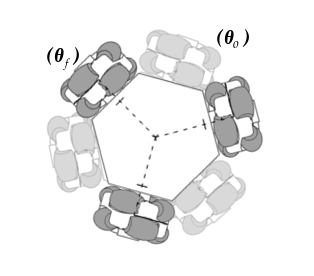
\includegraphics[width = 0.35\textwidth]{imagens/giro}
  \caption{Trajetória de giro.}
  \label{fig:giro}
\end{figure}

Na trajetória retilínea pura, se deseja validar a cinemática desenvolvida, e comprovar a eficiente compensação das não-linearidades dos atuadores e do algoritmo de limitação de velocidade. É a trajetória mostrada na Figura \ref{fig:reta}.

\begin{figure}[h]
  \centering
  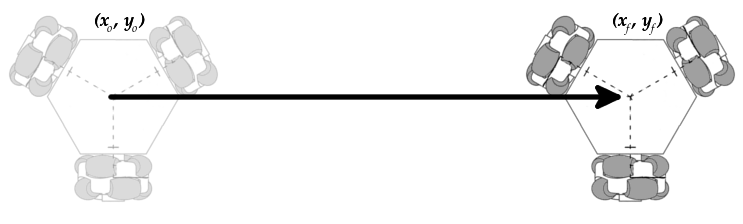
\includegraphics[width = 0.8\textwidth]{imagens/reta}
  \caption{Trajetória retilínea pura.}
  \label{fig:reta}
\end{figure}

Combinando ambas trajetórias, se deseja mover o robô da maneira mostrada na Figura \ref{fig:hibrida}. Para esta trajetória, é necessário recalcular as velocidades de acionamento a cada período de tempo, visto que o sistema referencial do robô é reorientado a cada instante pela rotação do chassi. No caso em que a odometria completa não está apresentando bons resultados, se pode acumular apenas a posição das rodas para a estimação da orientação atual do robô.

\begin{figure}[h]
  \centering
  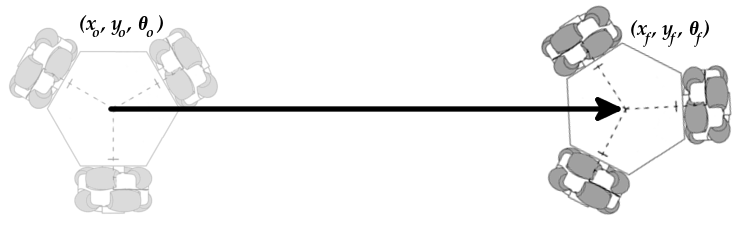
\includegraphics[width = 0.8\textwidth]{imagens/hibrida}
  \caption{Trajetória combinada.}
  \label{fig:hibrida}
\end{figure}

\subsection{Resultados}
\label{sec:resultados}

A implantação do sistema descrito nas seções anteriores é, de certa maneira, hierárquica: para que um subssistema de alto-nível funcione, os que estão abaixo dele devem estar funcionando também. Tal conceito pode ser visto na Figura \ref{fig:sistema}.

Os testes e validações ocorreram de maneira concomitante ao desenvolvimento do software e montagem da estrutura. Durante os testes de acionamento dos motores, se percebeu a presença de uma não linearidade do tipo ``zona-morta'', tendo sido realizado um ensaio para quantificar seu efeito. Os resultados de tal ensaio podem ser vistos na Figura \ref{fig:zonamorta}. Foi implementado um controlador proporcional para a velocidade, com ganho bastante baixo, de modo a tornar lenta a resposta do sistema. Foram então definidos \emph{setpoints} que propositalmente levassem a saturação dos \textit{drivers} dos atuadores. Na figura, se pode enxergar a zona morta em torno de $t=$1,5 s, quando a velocidade da roda se eleva repentinamente. Entre $t=$ 4 s e $t=$ 5 s, é realizado o comando de inversão da velocidade da roda, e para um intervalo de valores de acionamento em torno do eixo horizontal, não há movimento no eixo. Esta não linearidade é oriunda do atrito estático introduzido pelos componentes mecânicos responsáveis pela relação de redução.

\begin{figure}[h]
  \centering
  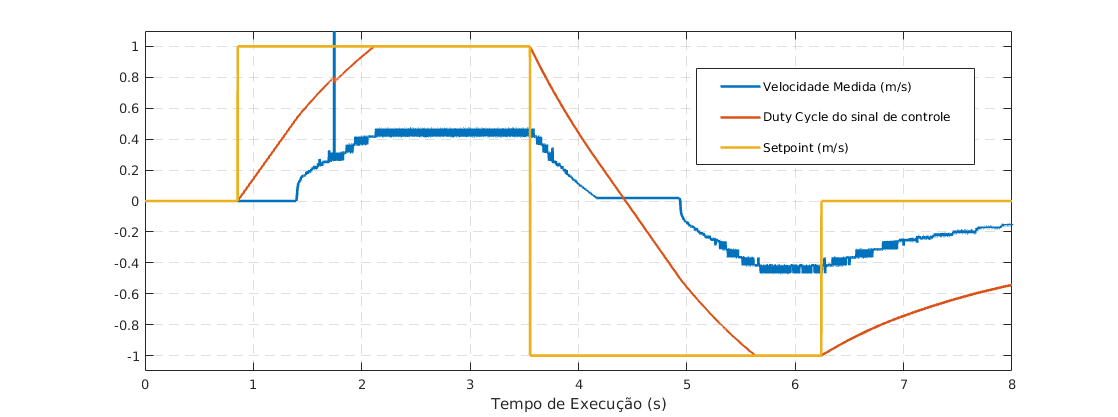
\includegraphics[width = \textwidth]{imagens/zonamorta}
  \caption{Análise da não-linearidade do tipo ``zona-morta'' presente nos motores utilizados.}
  \label{fig:zonamorta}
\end{figure}

O ensaio foi realizado simultaneamente com as três rodas, e como todas as leituras apresentaram resultados similares, apenas uma está mostrada no gráfico.

Uma consequência deste efeito foi verificada no acionamento do robô em trajetórias que exigem baixas velocidades de alguma das rodas. Esta situação pode ser vista na Figura \ref{fig:zm3rodas}, na qual se pode ver como os motores que devem operar em velocidades menores entram em operação com atraso, causando desvios de trajetória.

Foi aplicada a técnica descrita anteriormente \citep{cunha2001zm}. Pela análise dos dados mostrados na Figura \ref{fig:zm3rodas}, se pode perceber que a constante de compensação de zona morta é de aproximadamente 50\% do \textit{duty cycle} do PWM que aciona o \textit{driver}. Este método se mostrou bastante eficaz, conforme mostra a resposta simultânea de todos os motores na Figura \ref{fig:zm_comp}.

\begin{figure}[h!]
  \centering
  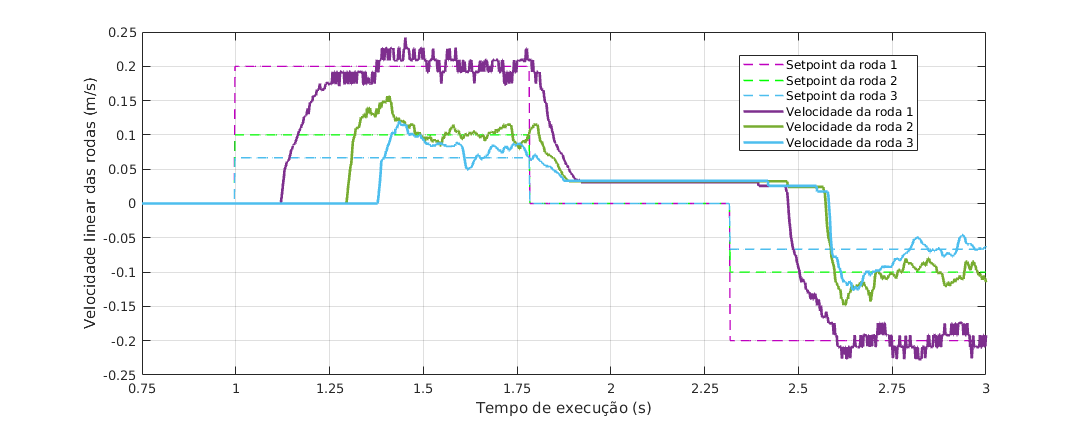
\includegraphics[width = \textwidth]{imagens/zm3rodas}
  \caption{Efeito da zona morta no acionamento das 3 rodas com velocidades distintas.}
  \label{fig:zm3rodas}
\end{figure}

\begin{figure}[h!]
  \centering
  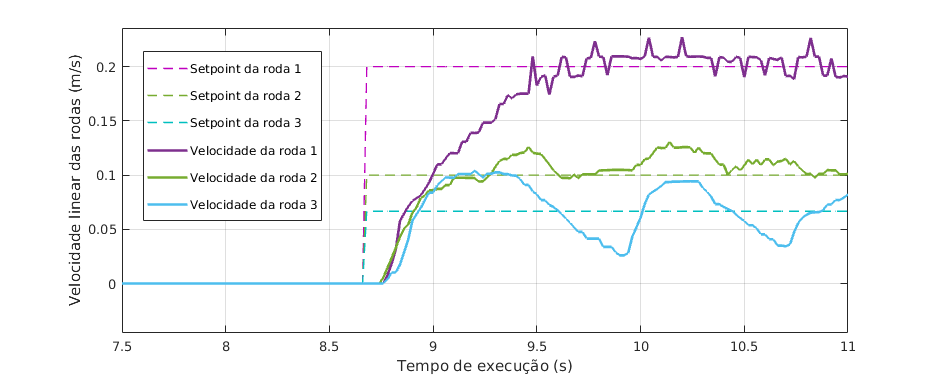
\includegraphics[width = \textwidth]{imagens/zmcomp}
  \caption{Não linearidade compensada -- acionamento quase simultâneo de todas as rodas.}
  \label{fig:zm_comp}
\end{figure}

Nota-se que no caso em que um motor deva operar com velocidades bastante baixas, como a roda 3 da figura, se introduz uma vibração em torno do \textit{setpoint}. Este efeito acontece pois quando o sinal de controle está muito perto do coeficiente de compensação, podem ocorrer ``pulos'' até o coeficiente de compensação do sentido oposto. Apesar de existirem técnicas para suavizar este efeito, as vibrações nas trajetórias realizadas não afetaram sgnificativamente o trajeto percorrido pelo robô.

Conforme mencionado anteriormente, o controlador de velocidade é do tipo proporcional (devido à necessidade de sua rápida implementação para continuar o desenvolvimento do restante do robô). Após alguns testes, se percebeu que  $K_P>20$ resulta em instabilidades (na forma de vibrações descontroladas no eixo do motor), e se optou por utilizar o ganho $K_P = 15$, que apresentou bom desempenho.

%\begin{figure}[h]
%  \centering
%  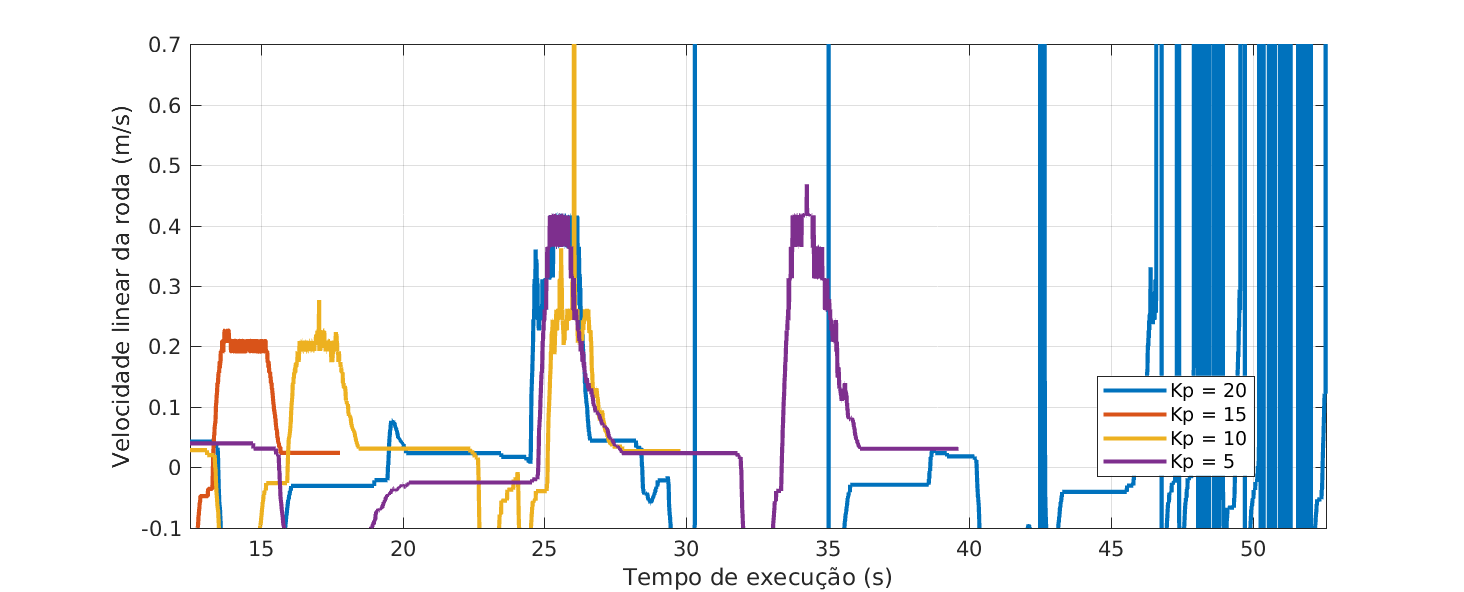
\includegraphics[width = \textwidth]{imagens/inst}
%  \caption{Resultados de operação aleatória do robô utilizando ganhos arbitrários.}
%  \label{fig:inst}
%\end{figure}

Outra verificação que foi feita durante a implementação foi a do fator de conversão da leitura da velocidade -- de pulsos/$\mu$s para m/s. Este fator, pelos parâmetros do robô, é de 534,18, no entanto se admite que possa haver alguma variação neste valor. Portanto, foi realizado um experimento para verificar a equivalência das unidades que o robô utiliza com referências externas. O robô foi operado em 3 trajetórias retílíneas: uma no eixo X, uma no eixo Y, e outra em X e Y, exatamente na diagonal do sistema de referência. O robô foi acionado com duas velocidades diferentes (0,15 m/s e 0,4 m/s) em cada trajetória, 5 vezes em cada velocidade, com um perfil de velocidade instantâneo, pelo tempo que resultaria na distância de 0,5 m se o robô estivesse adequadamente calibrado. O registro dos valores médios das distâncias medidas está apresentado na Tabela~\ref{tab:spd}.

\begin{table}
  \caption{Distância percorrida em trajetória retilínea com perfil de velocidade instantâneo.}
  \begin{tabular}{||c c c c||}
    \hline
     \textbf{Velocidade:} & \textbf{Distância em X:} & \textbf{Distância em XY:} & \textbf{Distância em Y:} \\ \hline\hline
     0,15 m/s        & 0,475 m    &  0,495 m     & 0,495 m    \\ \hline
     0,4 m/s         & 0,397 m    &  0,410 m     & 0,395 m    \\ \hline
  \end{tabular}
  \label{tab:spd}
\end{table}

Da tabela, se nota claramente que, quanto maior a velocidade, maior o erro na posição atingida. Tal resultado também foi observado durante a operação do robô em outras ocasiões, mostrando a grande influência da dinâmica do próprio robô. Poderia se argumentar que um controlador com tempo de ciclo menor pudesse responder de maneira mais ágil, porém o constatado no experimento está de acordo com \citet{lynch2017modern}: ``Na maioria das aplicações robóticas modernas, altas taxas de atualização de controladores apresentam benefícios limitados, devido às constantes de tempo associadas com a dinâmica do robô e do ambiente.''
%In most robotic applications, higher control update rates are of limited benefit, given time constants associated with the dynamics of the robot and environment.

%Tempo médio a cada chamada do loop de controle, em $\mu$s: 10000,03822
Também se percebeu que 0,15 m/s está perto do limite mínimo de velocidade desejado para uma operação confiável, devido aos efeitos introduzidos pela compensação de zona morta do atuador, recomendando-se assim a operação em torno de 0,25 m/s.

Ainda se analisando os resultados do experimento descrito acima, pode-se afirmar que as trajetórias realizadas pelo robô foram gravadas na superfície utilizando canetas hidrográficas nos furos do chassi destinados para tal. Na Figura \ref{fig:ef_zm} se pode visualizar as oscilações introduzidas pela compensação de zona morta para rodas que tenham que andar muito devagar, conforme mostrado também na Figura \ref{fig:zm_comp}.

\begin{figure}[h]
  \centering
  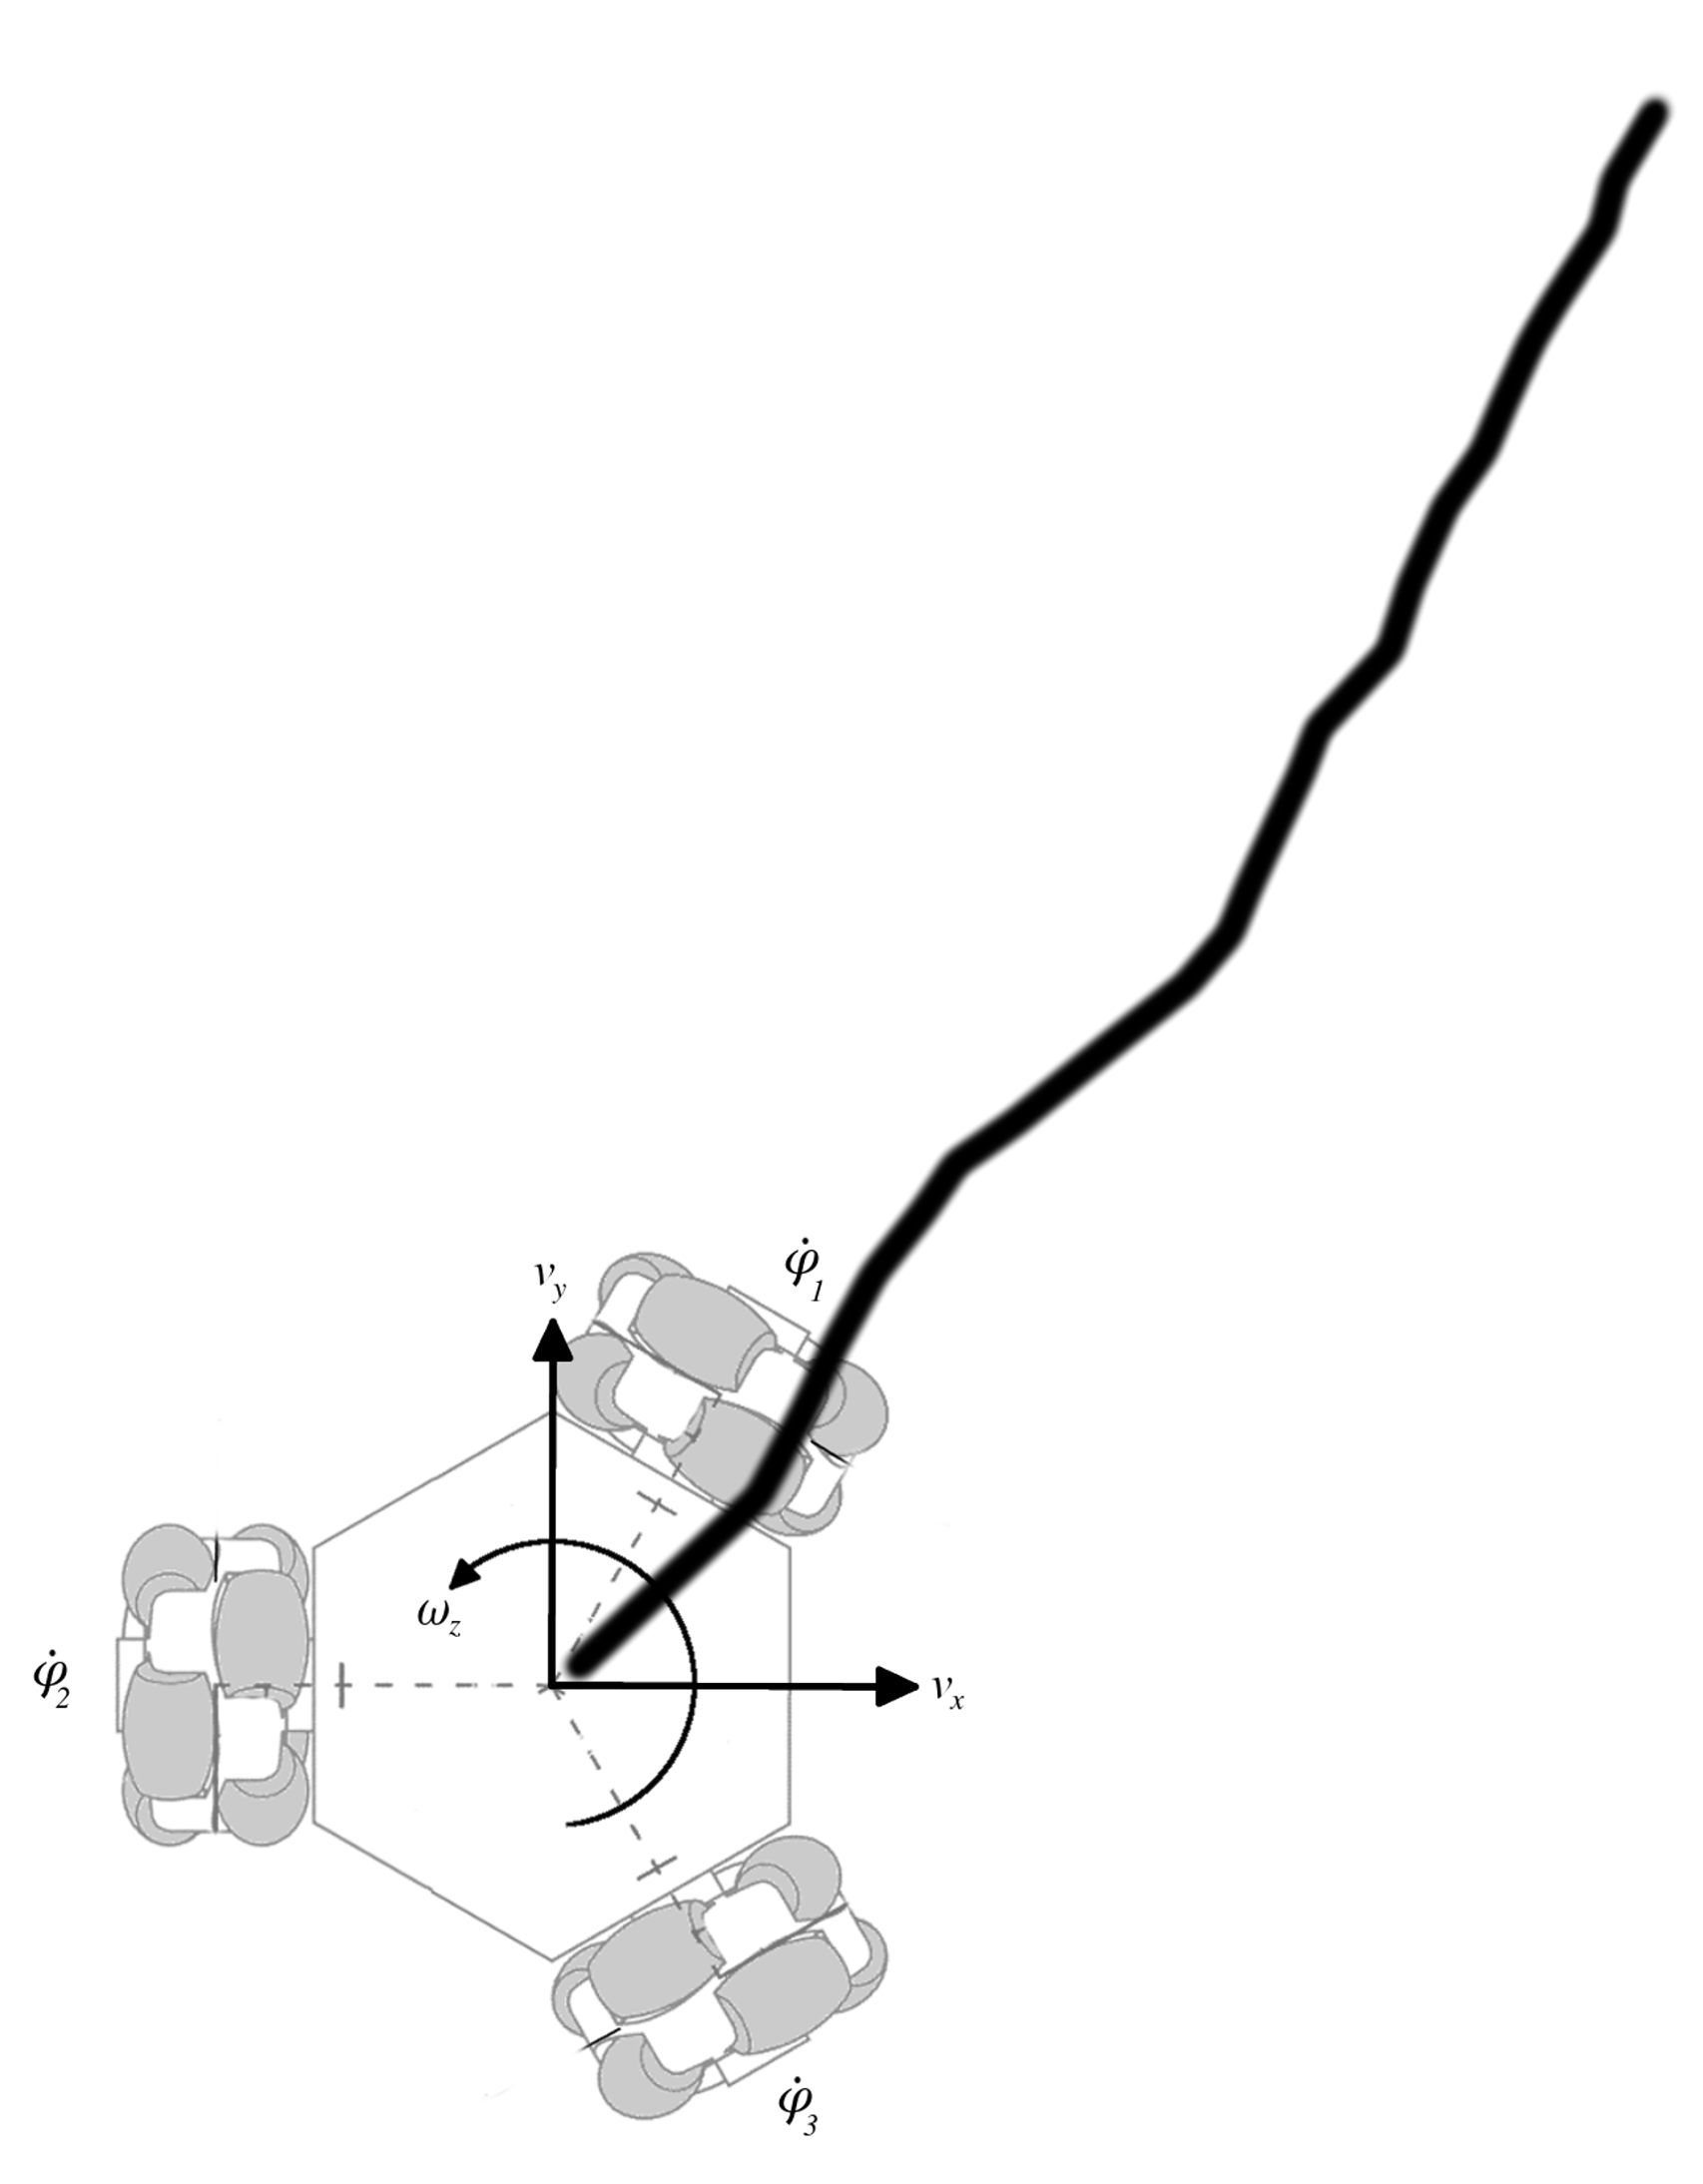
\includegraphics[width = 0.3\textwidth]{imagens/ef_zm}
  \caption{Trajetória real realizada pelo robô, em que a roda mais transversal ao caminho foi submetida a velocidades muito baixas (e não-nulas). A trajetória tem em torno de 0,5 m de comprimento.}
  \label{fig:ef_zm}
\end{figure}

Também é interessante observar a divergência das trajetórias em malha aberta. Na Figura \ref{fig:traj_y} se pode ver o ponto de partida do robô nos ensaios de trajetória reta no eixo Y com velocidade de 0,4 m/s. Para uma trajetória de 0,4 m, aproximadamente, se mediu em torno de 10 cm de desvio da trajetória desejada. Em trabalhos futuros, será realizado um estudo estatístico visando a avaliar se existe um erro sistemático no desvio, que possa permitir algum tipo de compensação.

\begin{figure}[h]
  \centering
  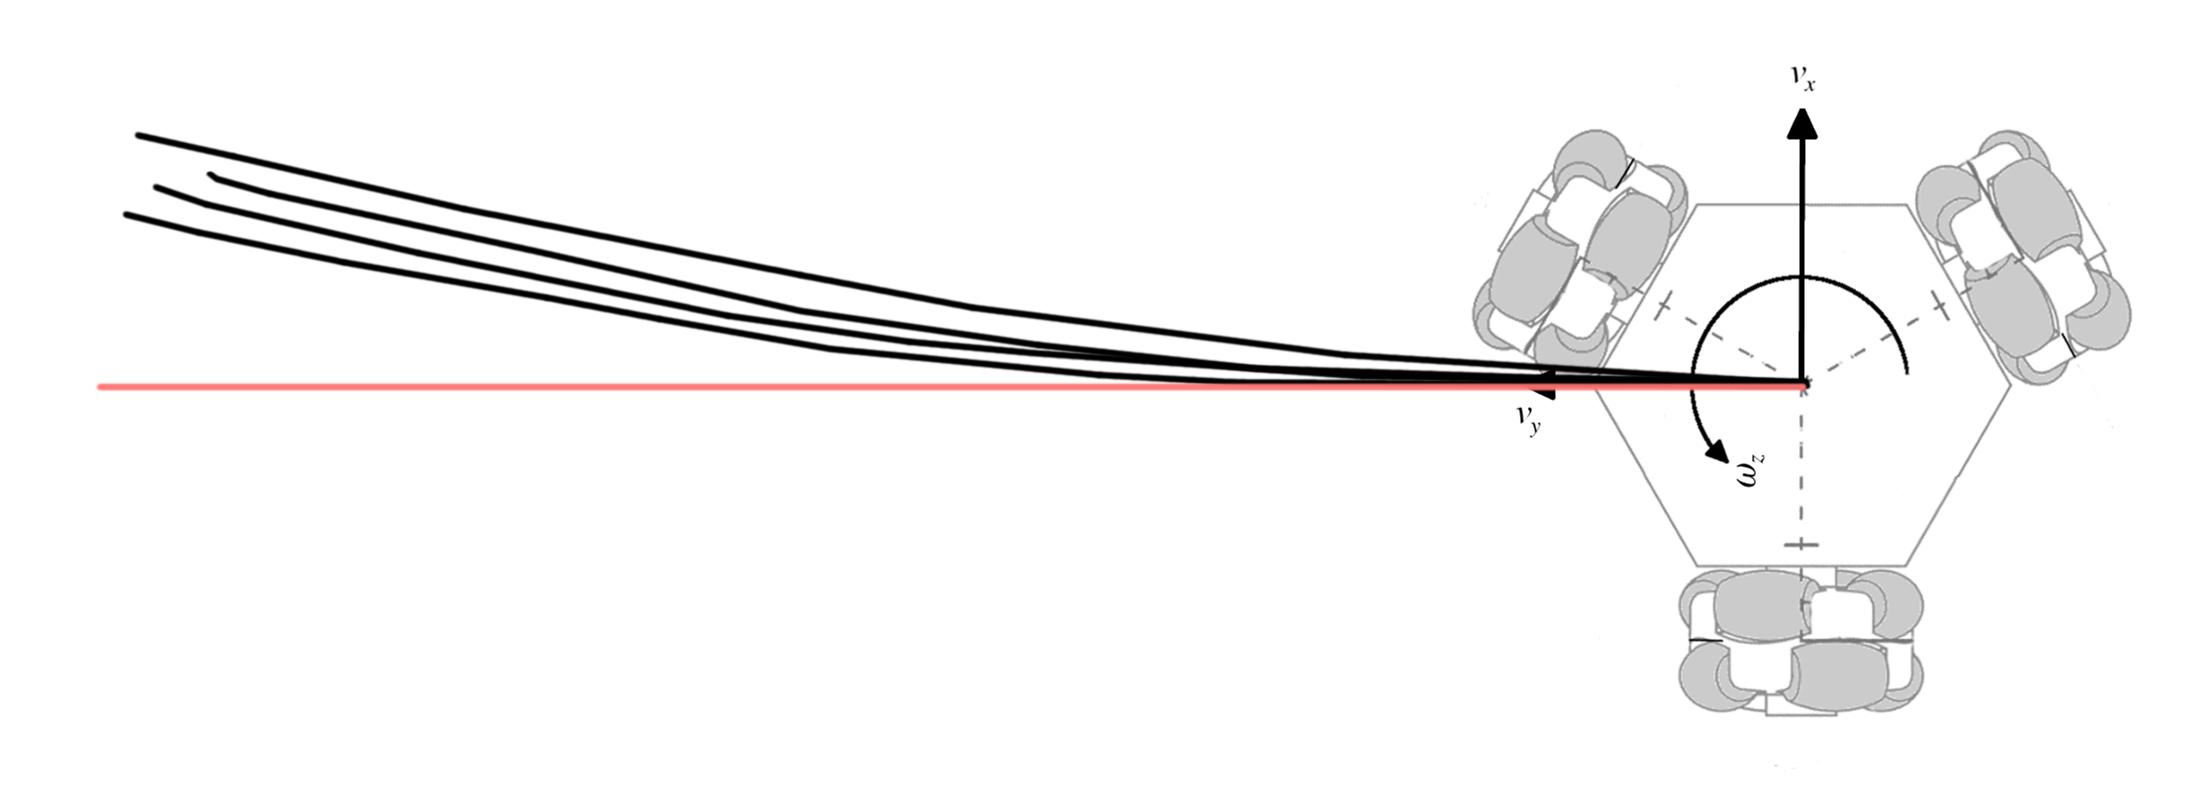
\includegraphics[width = 0.7\textwidth]{imagens/traj_y}
  \caption{Trajetórias em malha aberta, divergindo do ponto de origem. A trajetória desejada é a que está representada em vermelho.}
  \label{fig:traj_y}
\end{figure}

Após a implementação dos algoritmos de odometria, foram realizados testes do sistema, sendo que o equacionamento proposto por \citet{lynch2017modern} não apresentou resultados adequados. A causa disso ainda está sendo analisada. Foram também testadas as equações para o caso em que não se considera a velocidade angular. Sobre uma trajetória retilínea de aproximadamente 1,5 m no eixo X, se obtiveram valores razoáveis para a distância percorrida neste eixo: entre 1,2 m e 1,8 m. A variação entre os valores é grande, porém os experimentos se mostraram consistentes.

No eixo Y, perpendicular ao movimento, no entanto, foram contabilizadas distâncias variadas, na mesma ordem de grandeza que as do eixo X e para ambos os lados, com variação muito maior (de até 2 m, por exemplo). Tal resultado inviabilizou a utilização de algoritmos de controle de posição. Tal constatação é corroborada na mesma situação por \citet{siegwart2011introduction}: ``Note que a incerteza em Y cresce muito mais rápido do que na direção do movimento. Isso resulta da integração da incerteza a respeito da orientação do robô.''

O algoritmo de odometria completo foi abandonado, pois o uso de variáveis globais na biblioteca de cinemática faz com que a função de atualização da odometria altere os parâmetros utilizados para acionamento. Foi, no entanto, aproveitada a parte do algoritmo que identifica a orientação do robô, já que o ângulo $\theta$ pode ser obtido diretamente das variáveis que acumulam todos os pulsos dos \textit{encoders} desde o início da execução do programa. Este estimação se mostrou relativamente precisa para trajetórias circulares ou com alguns segmentos pequenos de reta. Não foi avaliada a estimativa do ângulo de orientação em trajetos mais complexos pois não se tem implementada nenhuma função de acionamento deste tipo.
